\documentclass{standalone}
\usepackage{tikz}
\usetikzlibrary{patterns, positioning}
\usepackage[sfdefault]{ClearSans} %% option 'sfdefault' activates Clear Sans as the default text font
\usepackage[T1]{fontenc}

\begin{document}
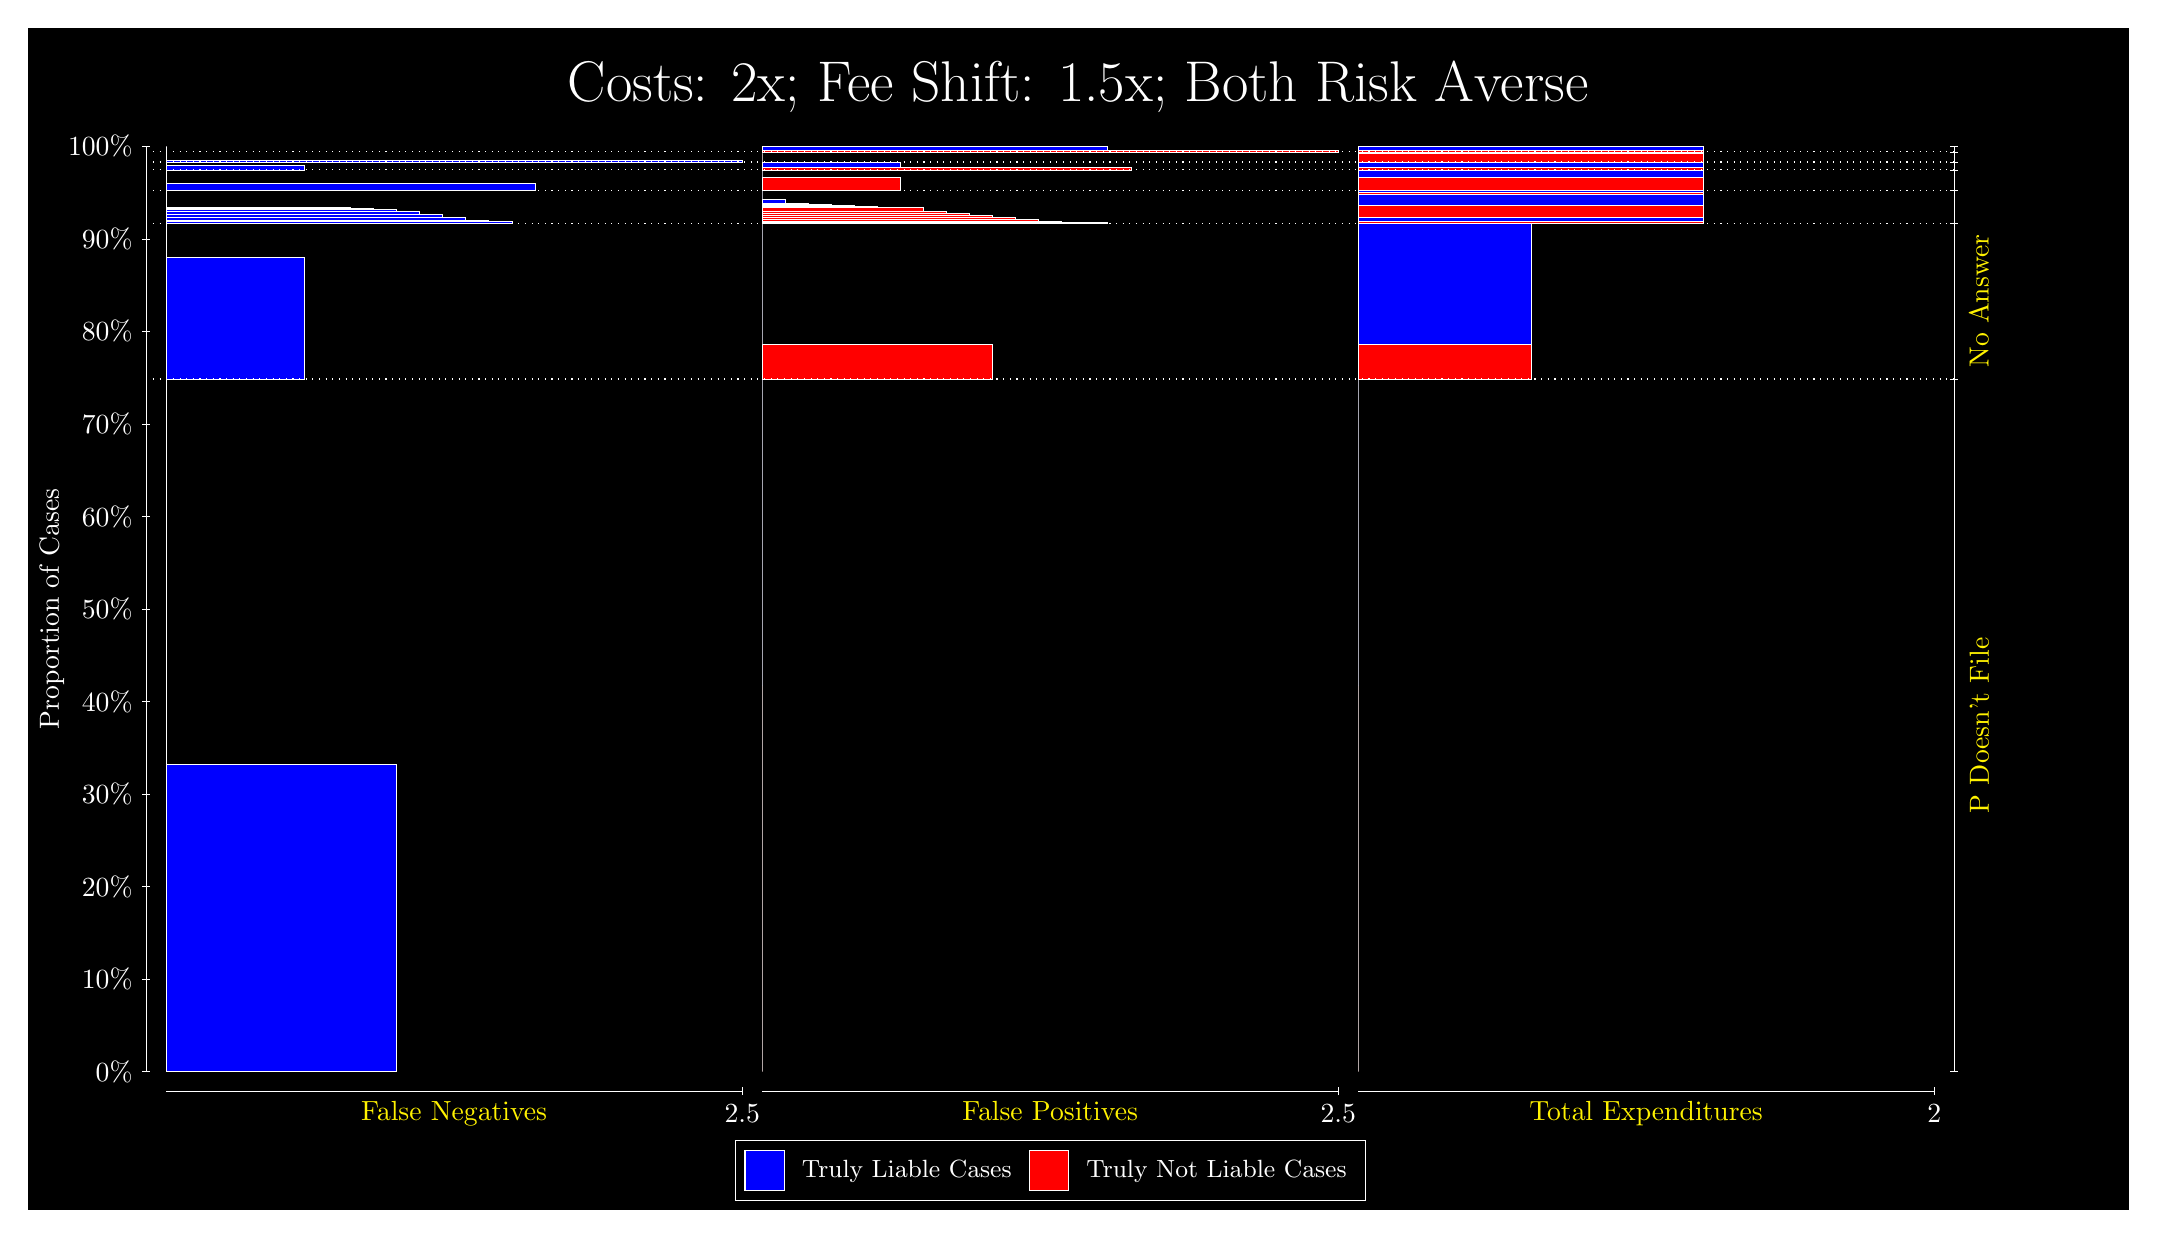
\begin{tikzpicture}
\draw[fill=black] (0,0) rectangle (26.667,15);
\draw[text=white] (0,13.5) rectangle (26.667,15) node[midway] {\huge Costs: 2x; Fee Shift: 1.5x; Both Risk Averse};
\draw[white, very thin] (1.5,1.75) -- (1.5,13.5);
\node[rotate=90, text=white, anchor=center] at (0.3, 7.625) {Proportion of Cases};
\draw[white, very thin] (1.45,1.75) -- (1.55,1.75);
\node[text=white, anchor=east] at (1.45, 1.75) {0\%};
\draw[white, very thin] (1.45,2.925) -- (1.55,2.925);
\node[text=white, anchor=east] at (1.45, 2.925) {10\%};
\draw[white, very thin] (1.45,4.1) -- (1.55,4.1);
\node[text=white, anchor=east] at (1.45, 4.1) {20\%};
\draw[white, very thin] (1.45,5.275) -- (1.55,5.275);
\node[text=white, anchor=east] at (1.45, 5.275) {30\%};
\draw[white, very thin] (1.45,6.45) -- (1.55,6.45);
\node[text=white, anchor=east] at (1.45, 6.45) {40\%};
\draw[white, very thin] (1.45,7.625) -- (1.55,7.625);
\node[text=white, anchor=east] at (1.45, 7.625) {50\%};
\draw[white, very thin] (1.45,8.8) -- (1.55,8.8);
\node[text=white, anchor=east] at (1.45, 8.8) {60\%};
\draw[white, very thin] (1.45,9.975) -- (1.55,9.975);
\node[text=white, anchor=east] at (1.45, 9.975) {70\%};
\draw[white, very thin] (1.45,11.15) -- (1.55,11.15);
\node[text=white, anchor=east] at (1.45, 11.15) {80\%};
\draw[white, very thin] (1.45,12.325) -- (1.55,12.325);
\node[text=white, anchor=east] at (1.45, 12.325) {90\%};
\draw[white, very thin] (1.45,13.5) -- (1.55,13.5);
\node[text=white, anchor=east] at (1.45, 13.5) {100\%};

\draw[white, very thin] (24.457,1.75) -- (24.457,13.5);
\draw[white, very thin] (24.407,1.75) -- (24.507,1.75);
\node[anchor=west] at (24.407, 1.75) {};
\draw[white, very thin] (24.407,10.545) -- (24.507,10.545);
\node[anchor=west] at (24.407, 10.545) {};
\draw[white, very thin] (24.407,12.524) -- (24.507,12.524);
\node[anchor=west] at (24.407, 12.524) {};
\draw[white, very thin] (24.407,12.936) -- (24.507,12.936);
\node[anchor=west] at (24.407, 12.936) {};
\draw[white, very thin] (24.407,13.201) -- (24.507,13.201);
\node[anchor=west] at (24.407, 13.201) {};
\draw[white, very thin] (24.407,13.301) -- (24.507,13.301);
\node[anchor=west] at (24.407, 13.301) {};
\draw[white, very thin] (24.407,13.43) -- (24.507,13.43);
\node[anchor=west] at (24.407, 13.43) {};
\draw[white, very thin] (24.407,13.5) -- (24.507,13.5);
\node[anchor=west] at (24.407, 13.5) {};

\draw[white, very thin, fill=blue] (1.75,1.75) rectangle (4.6775,5.6482);
\draw[white, very thin, fill=red] (1.75,5.6482) rectangle (1.75,10.545);
\draw[white, very thin, fill=blue] (1.75,10.545) rectangle (3.5065,12.088);
\draw[white, very thin, fill=red] (1.75,12.088) rectangle (1.75,12.524);
\draw[white, very thin, fill=blue] (1.75,12.524) rectangle (6.1413,12.55);
\draw[white, very thin, fill=blue] (1.75,12.55) rectangle (5.8486,12.559);
\draw[white, very thin, fill=blue] (1.75,12.559) rectangle (5.5558,12.595);
\draw[white, very thin, fill=blue] (1.75,12.595) rectangle (5.2631,12.636);
\draw[white, very thin, fill=blue] (1.75,12.636) rectangle (4.9703,12.677);
\draw[white, very thin, fill=blue] (1.75,12.677) rectangle (4.6775,12.699);
\draw[white, very thin, fill=blue] (1.75,12.699) rectangle (4.3848,12.715);
\draw[white, very thin, fill=blue] (1.75,12.715) rectangle (4.092,12.722);
\draw[white, very thin, fill=blue] (1.75,12.722) rectangle (3.7993,12.731);
\draw[white, very thin, fill=red] (1.75,12.731) rectangle (1.75,12.936);
\draw[white, very thin, fill=blue] (1.75,12.936) rectangle (6.4341,13.031);
\draw[white, very thin, fill=red] (1.75,13.031) rectangle (1.75,13.201);
\draw[white, very thin, fill=blue] (1.75,13.201) rectangle (3.5065,13.262);
\draw[white, very thin, fill=red] (1.75,13.262) rectangle (1.75,13.301);
\draw[white, very thin, fill=blue] (1.75,13.301) rectangle (9.0689,13.324);
\draw[white, very thin, fill=red] (1.75,13.324) rectangle (1.75,13.43);
\draw[white, very thin, fill=red] (1.75,13.43) rectangle (1.75,13.452);
\draw[white, very thin, fill=blue] (1.75,13.452) rectangle (1.75,13.5);
\draw[white, very thin, fill=red] (9.3189,1.75) rectangle (9.3189,6.6466);
\draw[white, very thin, fill=blue] (9.3189,6.6466) rectangle (9.3189,10.545);
\draw[white, very thin, fill=red] (9.3189,10.545) rectangle (12.246,10.981);
\draw[white, very thin, fill=blue] (9.3189,10.981) rectangle (9.3189,12.524);
\draw[white, very thin, fill=red] (9.3189,12.524) rectangle (13.71,12.532);
\draw[white, very thin, fill=red] (9.3189,12.532) rectangle (13.417,12.539);
\draw[white, very thin, fill=red] (9.3189,12.539) rectangle (13.125,12.554);
\draw[white, very thin, fill=red] (9.3189,12.554) rectangle (12.832,12.573);
\draw[white, very thin, fill=red] (9.3189,12.573) rectangle (12.539,12.6);
\draw[white, very thin, fill=red] (9.3189,12.6) rectangle (12.246,12.62);
\draw[white, very thin, fill=red] (9.3189,12.62) rectangle (11.954,12.655);
\draw[white, very thin, fill=red] (9.3189,12.655) rectangle (11.661,12.673);
\draw[white, very thin, fill=red] (9.3189,12.673) rectangle (11.368,12.73);
\draw[white, very thin, fill=blue] (9.3189,12.73) rectangle (10.783,12.738);
\draw[white, very thin, fill=blue] (9.3189,12.738) rectangle (10.49,12.746);
\draw[white, very thin, fill=blue] (9.3189,12.746) rectangle (10.197,12.762);
\draw[white, very thin, fill=blue] (9.3189,12.762) rectangle (9.9044,12.783);
\draw[white, very thin, fill=blue] (9.3189,12.783) rectangle (9.6116,12.825);
\draw[white, very thin, fill=blue] (9.3189,12.825) rectangle (9.3189,12.936);
\draw[white, very thin, fill=red] (9.3189,12.936) rectangle (11.075,13.106);
\draw[white, very thin, fill=blue] (9.3189,13.106) rectangle (9.3189,13.201);
\draw[white, very thin, fill=red] (9.3189,13.201) rectangle (14.003,13.24);
\draw[white, very thin, fill=blue] (9.3189,13.24) rectangle (11.075,13.301);
\draw[white, very thin, fill=red] (9.3189,13.301) rectangle (9.3189,13.407);
\draw[white, very thin, fill=blue] (9.3189,13.407) rectangle (9.3189,13.43);
\draw[white, very thin, fill=red] (9.3189,13.43) rectangle (16.638,13.452);
\draw[white, very thin, fill=blue] (9.3189,13.452) rectangle (13.71,13.5);
\draw[white, very thin, fill=red] (16.888,1.75) rectangle (16.888,6.6466);
\draw[white, very thin, fill=blue] (16.888,6.6466) rectangle (16.888,10.545);
\draw[white, very thin, fill=red] (16.888,10.545) rectangle (19.083,10.981);
\draw[white, very thin, fill=blue] (16.888,10.981) rectangle (19.083,12.524);
\draw[white, very thin, fill=red] (16.888,12.524) rectangle (21.279,12.551);
\draw[white, very thin, fill=blue] (16.888,12.551) rectangle (21.279,12.593);
\draw[white, very thin, fill=red] (16.888,12.593) rectangle (21.279,12.749);
\draw[white, very thin, fill=blue] (16.888,12.749) rectangle (21.279,12.891);
\draw[white, very thin, fill=red] (16.888,12.891) rectangle (21.279,12.913);
\draw[white, very thin, fill=blue] (16.888,12.913) rectangle (21.279,12.936);
\draw[white, very thin, fill=red] (16.888,12.936) rectangle (21.279,13.106);
\draw[white, very thin, fill=blue] (16.888,13.106) rectangle (21.279,13.201);
\draw[white, very thin, fill=red] (16.888,13.201) rectangle (21.279,13.24);
\draw[white, very thin, fill=blue] (16.888,13.24) rectangle (21.279,13.301);
\draw[white, very thin, fill=red] (16.888,13.301) rectangle (21.279,13.407);
\draw[white, very thin, fill=blue] (16.888,13.407) rectangle (21.279,13.43);
\draw[white, very thin, fill=red] (16.888,13.43) rectangle (21.279,13.452);
\draw[white, very thin, fill=blue] (16.888,13.452) rectangle (21.279,13.5);
\draw[white, dotted] (1.5,10.545) -- (24.457,10.545);
\draw[white, dotted] (1.5,12.524) -- (24.457,12.524);
\draw[white, dotted] (1.5,12.936) -- (24.457,12.936);
\draw[white, dotted] (1.5,13.201) -- (24.457,13.201);
\draw[white, dotted] (1.5,13.301) -- (24.457,13.301);
\draw[white, dotted] (1.5,13.43) -- (24.457,13.43);
\draw[white, very thin] (1.75,1.5) -- (9.0689,1.5);
\node[text=yellow, anchor=north] at (5.4094, 1.5) {False Negatives};
\draw[white, very thin] (9.0689,1.45) -- (9.0689,1.55);
\node[text=white, anchor=north] at (9.0689, 1.45) {2.5};

\draw[white, very thin] (9.3189,1.5) -- (16.638,1.5);
\node[text=yellow, anchor=north] at (12.978, 1.5) {False Positives};
\draw[white, very thin] (16.638,1.45) -- (16.638,1.55);
\node[text=white, anchor=north] at (16.638, 1.45) {2.5};

\draw[white, very thin] (16.888,1.5) -- (24.207,1.5);
\node[text=yellow, anchor=north] at (20.547, 1.5) {Total Expenditures};
\draw[white, very thin] (24.207,1.45) -- (24.207,1.55);
\node[text=white, anchor=north] at (24.207, 1.45) {2};

\node[text=yellow, centered, rotate=90] at (24.777, 6.1474) {P Doesn't File};
\node[text=yellow, centered, rotate=90] at (24.777, 11.535) {No Answer};






\draw (12.978300999999998,1.5) node[draw=none] (baseCoordinate) {};
\begin{scope}[align=center]
        \matrix[scale=0.5, draw=white, below=0.5cm of baseCoordinate, nodes={draw}, column sep=0.1cm]{
            \node[rectangle, draw, minimum width=0.5cm, minimum height=0.5cm, fill=blue] {}; &
            \node[draw=none, font=\small, text=white] (B) {Truly Liable Cases}; &
            \node[rectangle, draw, minimum width=0.5cm, minimum height=0.5cm, fill=red] {}; &
            \node[draw=none, font=\small, text=white] (B) {Truly Not Liable Cases}; \\
            };
\end{scope}

\end{tikzpicture}
\end{document}